% Preliminary study: LLM-guided program evolution on the continuous Erdos
% minimum overlap problem. Numbers are a snapshot of runs that were cut short
% by exhaustion of API credit; see Section 5.
%
% NOTE TO AUTHOR: fill in \author{...}. The bibliography entries were written
% from memory and have NOT been checked against the sources -- verify them.
\documentclass[11pt]{article}

\usepackage[margin=1in]{geometry}
\usepackage{amsmath,amssymb,amsthm}
\usepackage{graphicx}
\usepackage{booktabs}
\usepackage{hyperref}
\usepackage{caption}

\graphicspath{{figures/}}

\newtheorem{proposition}{Proposition}

\newcommand{\Cmax}{C_{\max}}
\newcommand{\R}{\mathbb{R}}

\title{Evolving Step Functions for the Erd\H{o}s Minimum Overlap Problem\\
with LLM-Guided Program Search: A Preliminary Study}
\author{[Author name]}
\date{\today}

\begin{document}
\maketitle

\begin{abstract}
The Erd\H{o}s minimum overlap problem asks how evenly the integers
$1,\dots,2n$ can be split into two equal halves so that no difference occurs
too often. Its continuous reformulation asks for a step function
$f:[0,2]\to[0,1]$ with $\int f = 1$ minimising
$\max_k \int f(x)\,(1-f(x+k))\,dx$; the best published upper bound we targeted
is $0.380871$. We report a preliminary study of LLM-guided program evolution
(ShinkaEvolve) on this problem. We build an exact, independently verified
scorer and four evolution setups that differ in what is evolved: the solution,
the optimiser, the parametrisation, or the resolution. With a single seed per
setup, and runs ended early by exhaustion of API credit, the best construction
reached $0.38175$: an improvement of $0.0008$ over its own seed, but still
$0.0009$ above the published bound. No setup improved the record. We also
document an evaluation pitfall that silently invalidated an initial set of
runs, and a cost analysis showing that spend is dominated by model output, a
premium model, and prompt overhead. All results are preliminary and are not
statistically established.
\end{abstract}

\section{Introduction}

Erd\H{o}s' minimum overlap problem~\cite{erdos55} asks for a partition of
$\{1,\dots,2n\}$ into two sets $A$ and $B$ of size $n$ that minimises the
largest number of solutions of $a - b = k$ over all integers $k$. Writing
$M(n)$ for this minimum, the limit $M(n)/n$ is bounded above by evaluating a
continuous relaxation, attributed to Swinnerton-Dyer, in which the sets are
replaced by a density $f$ (see Haugland~\cite{haugland16}). Every admissible
$f$ therefore certifies an upper bound on the limiting constant, and progress
on the problem takes the form of ever-better step functions.

Recently, LLM-guided evolutionary program search, as in
AlphaEvolve~\cite{alphaevolve} and the open-source
ShinkaEvolve~\cite{shinka}, has produced improved constructions for several
extremal problems. This note asks a modest question: if we wrap the continuous
overlap problem in ShinkaEvolve, which design choices matter, and what does it
cost? We contribute (i) a verified exact scorer, (ii) four evolution setups and
a first, single-seed comparison, (iii) an account of an evaluation pitfall that
invalidated early runs, and (iv) a token-level cost breakdown.

\section{Problem and Scorer}

\subsection{Formulation}

Let $f:[0,2]\to[0,1]$ be measurable with $\int_0^2 f = 1$, and let $g = 1-f$ on
$[0,2]$, extended by $0$ outside. Define the overlap at shift $k\in\R$ by
\begin{equation}
  C_f(k) \;=\; \int_{\R} f(x)\,g(x+k)\,dx ,
  \qquad
  \Cmax(f) \;=\; \sup_{k} C_f(k).
\end{equation}
The task is to minimise $\Cmax(f)$. We represent $f$ as $n$ equal-width steps
with heights $h_0,\dots,h_{n-1}\in[0,1]$, width $w=2/n$, and
$\sum_i h_i\,w = 1$.

\subsection{Exactness of grid evaluation}

\begin{proposition}
For a step function on a uniform grid of width $w$, $C_f$ is piecewise linear
in $k$ with breakpoints at integer multiples of $w$. Hence
$\sup_k C_f(k)$ is attained at a grid shift $k=jw$.
\end{proposition}

\begin{proof}
Let $k=(j+\theta)w$ with $j\in\mathbb{Z}$ and $\theta\in[0,1)$, and let
$g_i = 1-h_i$ for $0\le i<n$ and $g_i=0$ otherwise. For $x$ in cell $i$ the
point $x+k$ falls in cells $i+j$ and $i+j+1$ with measures $(1-\theta)w$ and
$\theta w$ respectively, so
$\int_{\text{cell } i} g(x+k)\,dx = w\big[(1-\theta)g_{i+j}+\theta g_{i+j+1}\big]$.
Summing over $i$ with $f=h_i$ on cell $i$ gives
$C_f(k)=(1-\theta)C_j+\theta C_{j+1}$, where $C_j=C_f(jw)$. A continuous
piecewise linear function attains its maximum at a breakpoint.
\end{proof}

The scorer therefore evaluates every grid lag with a single FFT
cross-correlation; no subsampling of shifts is needed or used.

\subsection{Verification}

Each program is scored by recomputing $\Cmax$ from its returned heights; the
evaluator rejects a program whose self-reported value differs from the
recomputed value by more than $10^{-6}$, and rejects heights outside $[0,1]$
or with $|\int f - 1|>10^{-4}$. We additionally verified the scorer itself
(Table~\ref{tab:verify}); the script is part of the repository.

\begin{table}[h]
\centering
\caption{Scorer verification (all checks pass).}
\label{tab:verify}
\begin{tabular}{p{9.2cm}l}
\toprule
Check & Result \\
\midrule
Hand-worked cases ($[1,0]\to1$, $[0,1]\to1$, $[1,0,0,1]\to0.5$) & exact \\
FFT scorer vs.\ plain loops, warm start ($n=600$) & max abs.\ diff.\ $0$ \\
FFT scorer vs.\ plain loops, 25 random arrays & max abs.\ diff.\ $2.2\times10^{-16}$ \\
Overlap at non-grid shifts vs.\ linear interpolation & max abs.\ err.\ $2.8\times10^{-16}$ \\
Same function on a $7\times$ finer grid & identical to 8 decimals \\
\bottomrule
\end{tabular}
\end{table}

\paragraph{Caveats.}
(1) The scorer omits lag $0$. By continuity the supremum over $k\neq0$ also
approaches $C_f(0)=\int f(1-f)$, so omission could in principle under-score a
candidate with large $C_f(0)$. For our warm start $C_f(0)=0.3297$, below
$\Cmax=0.3829$, so it is harmless there; we did not change the scorer mid-run
so that scores stay comparable. (2) The mass tolerance of $10^{-4}$ exceeds
the improvements of interest. On the warm start, rescaling the mass by up to
$\approx8\times10^{-5}$ in either direction made the score \emph{worse}, so it
was not exploitable there, but any final claim should be re-scored after exact
normalisation.

\section{Evolution Setups}

We use ShinkaEvolve~\cite{shinka} with island populations, a UCB1 bandit over
the available models (Setup~D uses a single model, so no bandit), a novelty
filter based on code embeddings, and periodic meta-recommendations. The four
setups differ in what the program under evolution produces
(Table~\ref{tab:setups}).

\begin{table}[h]
\centering
\caption{The four setups. $n$ is the number of steps. Caps are API-cost limits
per run.}
\label{tab:setups}
\small
\begin{tabular}{llllll}
\toprule
 & Evolved component & $n$ & Islands/archive & Models & Cap \\
\midrule
A & start heights + SLSQP polisher & 600 & 2 / 40 & Sonnet 5, Haiku 4.5 & \$5 \\
B & the optimiser itself & 2048 & 4 / 60 & Sonnet 5, Opus 5 & \$6 \\
C & the parametrisation & 256--4096 & 6 / 100 & Haiku, Sonnet, Opus & \$6 \\
D & rung 1 of a resolution ladder & 600 & 3 / 50 & Sonnet 5 & \$3 \\
\bottomrule
\end{tabular}
\end{table}

\paragraph{Seeds.}
A and D start from a warm start obtained by eight random-restart SLSQP
optimisations at $n=600$ ($\Cmax=0.382908$). This is \emph{self-derived}, not
the published solution, whose heights we could not recover from the source
papers. B starts from the same warm start, resampled to $n=2048$, with a
deliberately naive single-shift subgradient descent as the optimiser to be
improved. C starts from a smooth symmetric Fourier parametrisation, a
structurally different but much weaker seed ($0.4248$), so C is not a
like-for-like comparison with A, B, D. D is only the first rung of an intended
four-rung ladder ($n=600\to2048\to8192\to16384$); the later rungs were not
run.

\section{Protocol and Pitfalls}

\paragraph{Invalidated first runs.}
ShinkaEvolve copies only the evolved program file into an isolated folder per
generation. Our first seeds loaded the warm start from a sibling \texttt{.npy}
file, which did not exist there. Setup~A and D silently fell back to a
sine-wave start (generation~0 scored $0.4203$ instead of the validated
$0.3826$); B loaded without a fallback and would crash. Nothing logged an error
for A and D. The bug was caught because the generation-0 score disagreed with a
standalone validation of the same seed. The fix embeds the warm start in each
seed file, outside the evolvable region. \textbf{Only runs started after the
fix are reported here.}

\paragraph{Infrastructure failures.}
An expired API key (HTTP 401) and an empty credit balance (HTTP 400) do not
crash a run: calls are retried while generation~0, which needs no model call,
scores normally. A run can therefore look healthy while making no progress. We
now treat the existence of programs at generation $\ge1$ as the health check.
The reported runs were cut short when the credit balance was exhausted.

\section{Results}

Table~\ref{tab:results} and Figure~\ref{fig:cost} show a snapshot of the valid
run set. Because the runs were interrupted by credit exhaustion at different
points, final scores are \emph{not} comparable at equal budget; we therefore
plot best score against cumulative spend.

\begin{table}[h]
\centering
\caption{Snapshot of the valid run set (one seed per setup). Scores are
$\Cmax$; lower is better. Spend counts stored programs only. The published
bound is $0.380871$.}
\label{tab:results}
\small
\begin{tabular}{lrrrrrr}
\toprule
Setup & Seed & Best & Gain & Programs (valid) & Spend & Gap to bound \\
\midrule
A & 0.38256 & \textbf{0.38175} & 0.00081 & 10 (9) & \$0.74 & 0.00088 \\
B & 0.38420 & 0.38340 & 0.00080 & 22 (19) & \$4.18 & 0.00253 \\
C & 0.42483 & 0.42483 & 0 & 10 (4) & \$0.20 & 0.04396 \\
D & 0.38271 & 0.38237 & 0.00034 & 4 (2) & \$0.11 & 0.00150 \\
\bottomrule
\end{tabular}
\end{table}

\begin{figure}[h]
\centering
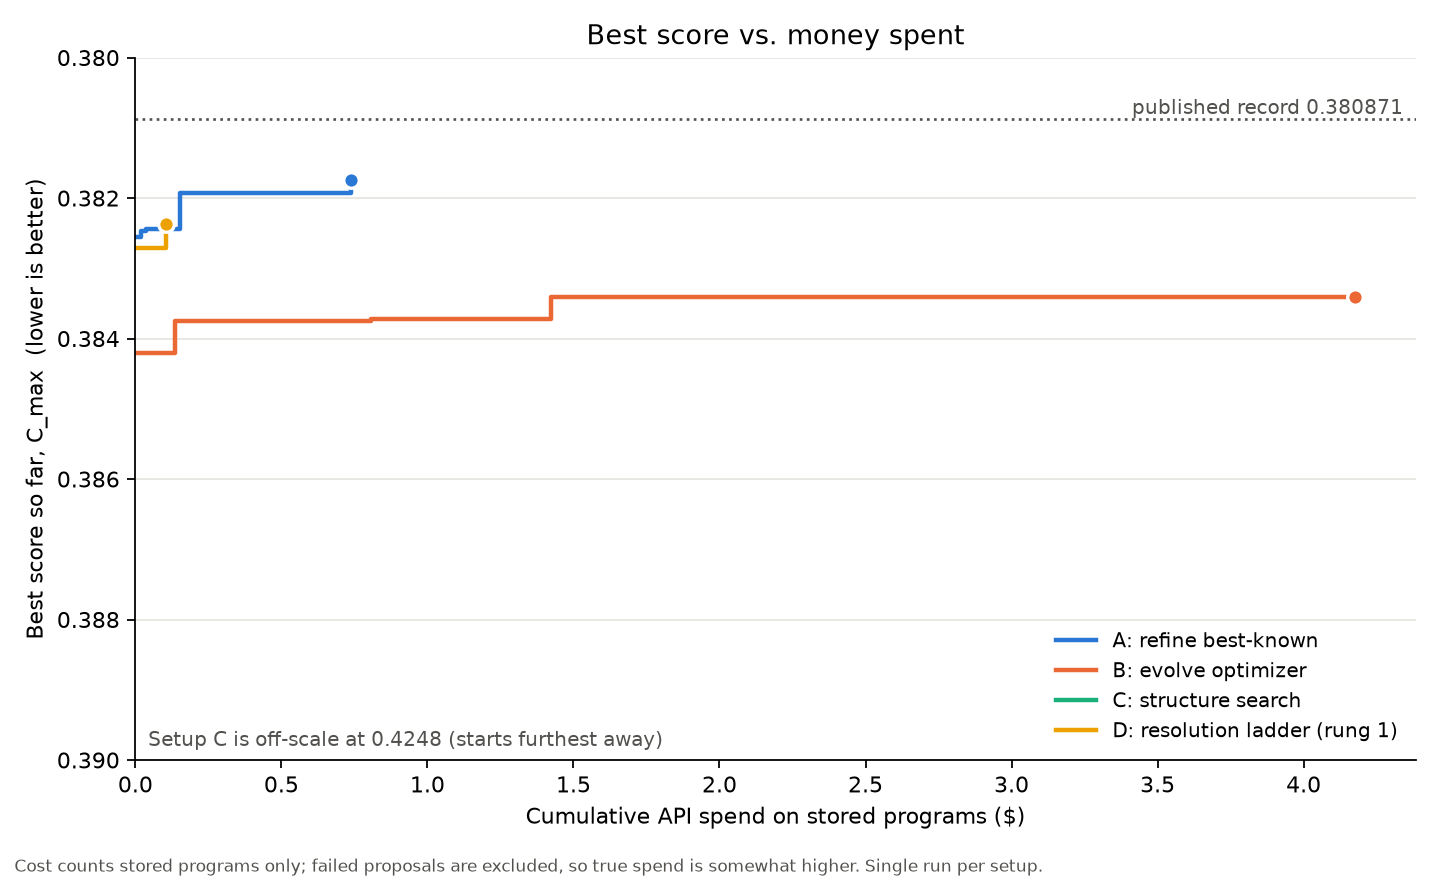
\includegraphics[width=0.85\textwidth]{cost_curves.png}
\caption{Best score against cumulative API spend. Setup C is off-scale
($0.4248$). Cost counts stored programs only; failed proposals are excluded,
so true spend is somewhat higher.}
\label{fig:cost}
\end{figure}

\paragraph{Observations (descriptive only).}
Setups that refine a strong warm start (A, D) gained $0.0008$ and $0.0003$
within a dollar. B gained a similar amount to A but spent about $5.6\times$
more. C produced no improvement and only 4 valid programs of 10. No setup
improved the published bound. With a single seed per setup and unequal spend,
we draw no ranking conclusion.

\begin{figure}[h]
\centering
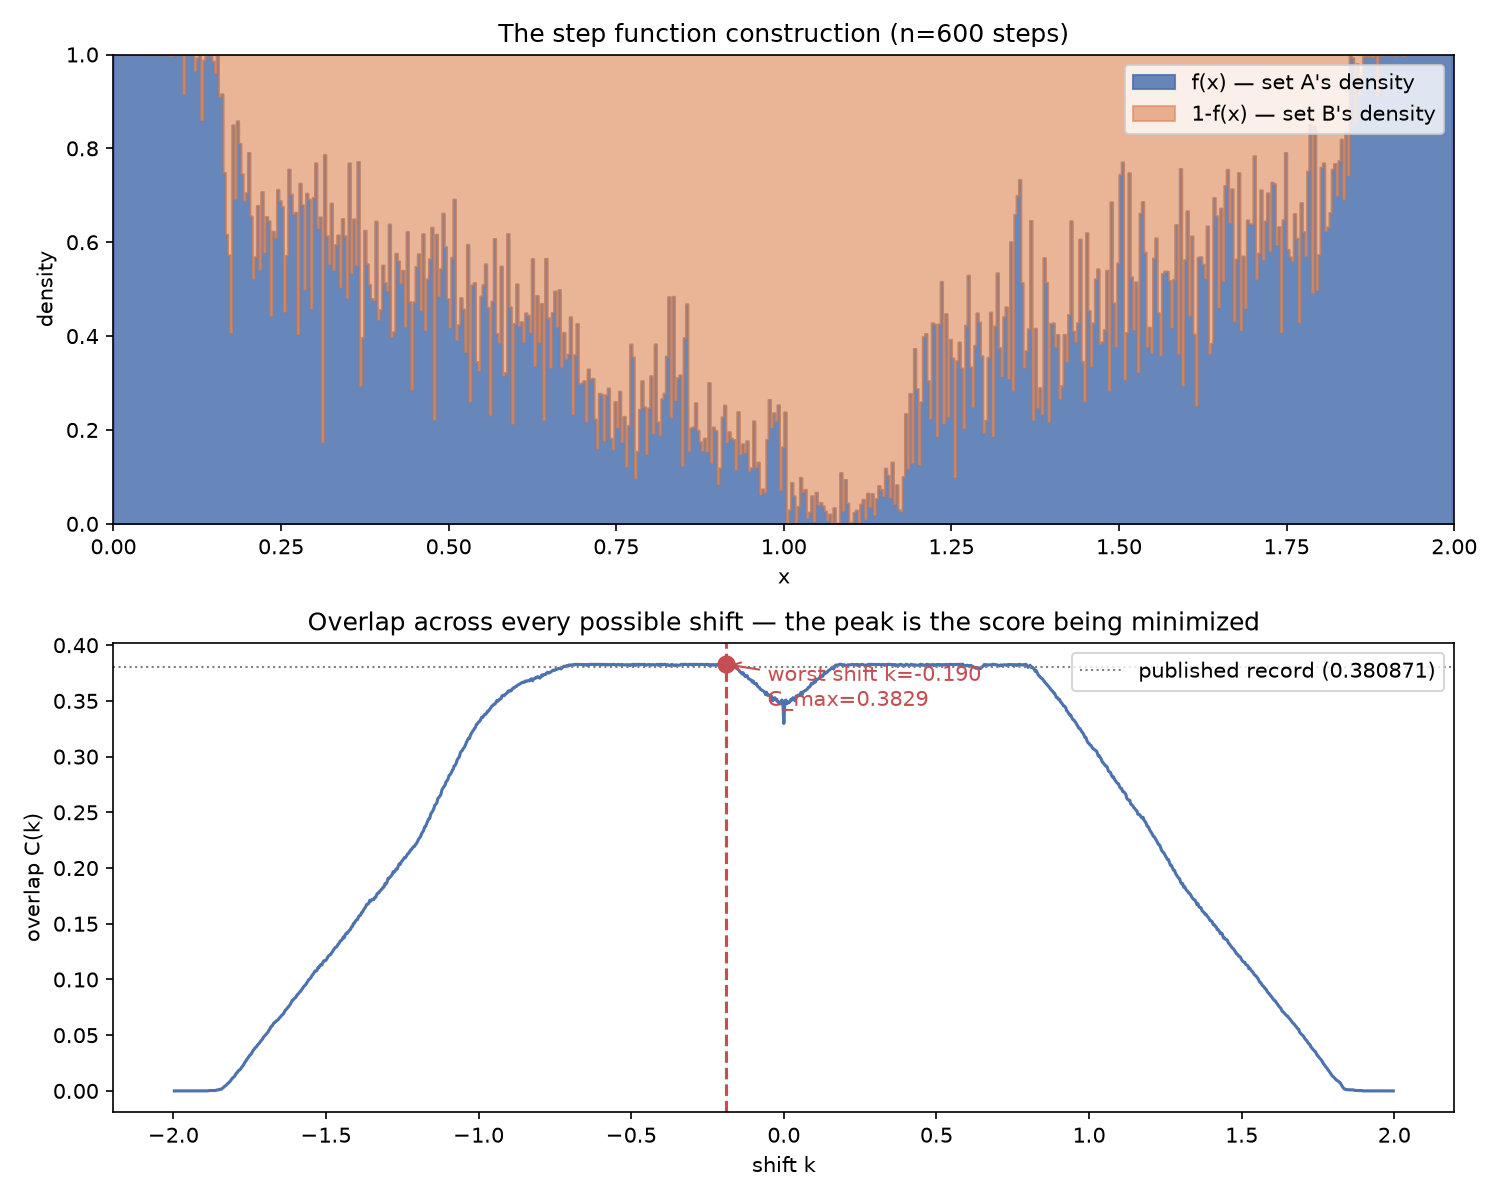
\includegraphics[width=0.85\textwidth]{overlap_visualization.png}
\caption{The $n=600$ warm start: step function $f$ and its overlap curve
$C_f(k)$ across all shifts; the peak is the score being minimised
($\Cmax=0.3829$).}
\label{fig:construction}
\end{figure}

\section{Cost Analysis}

The databases record input and output tokens per call. Over 30 proposal calls
at the time of analysis (Table~\ref{tab:cost}):

\begin{itemize}
\item \textbf{Output dominates.} Output tokens were 64\% of proposal cost, at
an average of 7{,}500 output tokens per call. The visible answers are only a
few thousand characters, so most output appears to be hidden reasoning that is
not stored (the recorded thinking-token field was $0$); this is an inference.
\item \textbf{Premium model.} Opus~5 cost about $\$0.47$ per call against
$\$0.14$ for Sonnet~5. Three Opus calls accounted for roughly a third of
proposal spend.
\item \textbf{Prompt overhead from embedding the warm start.} The embedded
base64 warm start is about half of every prompt by size and is repeated for
each inspiration program shown. We estimate this at 11--18\% of proposal cost
(assuming 3--5k tokens per copy). This is a side effect of our fix for the
missing-file bug.
\item \textbf{Hidden spend.} B made 57 successful API calls for about 22 stored
programs; novelty checks, summaries and failed proposals cost money but leave
no stored program, so stored cost understates true spend.
\end{itemize}

\begin{table}[h]
\centering
\caption{Per-call proposal cost by model (30 calls).}
\label{tab:cost}
\small
\begin{tabular}{lrrr}
\toprule
Model & Calls & Avg.\ cost & Avg.\ output tokens \\
\midrule
Haiku 4.5 & 7 & \$0.025 & 3{,}059 \\
Sonnet 5 & 20 & \$0.136 & 8{,}205 \\
Opus 5 & 3 & \$0.466 & 13{,}577 \\
\bottomrule
\end{tabular}
\end{table}

\section{Limitations and Next Steps}

\paragraph{Threats to validity.}
One seed per setup; unequal spend and resolutions across setups; a self-derived
rather than published warm start; interrupted runs; the scorer caveats in
Section~2.3; and Setup~D covering only one rung.

\paragraph{No non-LLM control.}
We did not test whether a compute-matched classical optimiser (the same
polisher with random restarts) matches the evolved runs. This control is the
most important missing experiment, since without it the contribution of the
LLM is unestablished.

\paragraph{Planned follow-ups.}
(i) The non-LLM control above. (ii) Multiple seeds at equal budget.
(iii) Seeding with a minimax-appropriate solver (e.g.\ sequential linear
programming on the ``ceiling'' form), and evolving its settings.
(iv) A feedback ablation: Setup~A with the evaluator reporting which shifts
are tied for the maximum. (v) Warm starting from the published construction,
if recoverable. (vi) Reducing prompt overhead and removing the premium model
to lower cost per program.

\section{Conclusion}

A verified exact scorer and four evolution setups were built and a first,
single-seed comparison obtained. The best construction reached $0.38175$,
improving on its own seed but not on the published bound of $0.380871$. The
main findings so far are methodological: silent fallback paths can invalidate
runs without any error, a run can appear healthy while making no progress, and
cost is dominated by model output and a premium model. The comparative
questions remain open pending equal-budget, multi-seed runs and a non-LLM
control.

\appendix
\section{Brute-Force Sanity Check for Small Universes}

For universe size $N$ and a set $A$ of size $s$ (with $B$ the complement), let
$z(N,s)$ be the minimum over $A$ of the largest number of pairs $(a,b)$ with
$a-b=k$. Exhaustive enumeration for $N\le10$ gives Table~\ref{tab:small}. The
balanced cases $N=2n$, $s=n$ give $1,1,2,2,3$ for $n=1,\dots,5$, matching the
known values of the original problem.

\begin{table}[h]
\centering
\caption{Minimal overlap $z(N,s)$ by exhaustive search; blank where $s\ge N$.}
\label{tab:small}
\small
\begin{tabular}{r|rrrrrrrrr}
\toprule
$N\backslash s$ & 1 & 2 & 3 & 4 & 5 & 6 & 7 & 8 & 9 \\
\midrule
2 & 1 & & & & & & & & \\
3 & 1 & 1 & & & & & & & \\
4 & 1 & 1 & 1 & & & & & & \\
5 & 1 & 1 & 1 & 1 & & & & & \\
6 & 1 & 1 & 2 & 1 & 1 & & & & \\
7 & 1 & 1 & 2 & 2 & 1 & 1 & & & \\
8 & 1 & 1 & 2 & 2 & 2 & 1 & 1 & & \\
9 & 1 & 1 & 2 & 2 & 2 & 2 & 1 & 1 & \\
10 & 1 & 1 & 2 & 2 & 3 & 2 & 2 & 1 & 1 \\
\bottomrule
\end{tabular}
\end{table}

\section{Reproducibility}

Code and results: \url{https://github.com/van3gue/EvolutionaryMathematics}.
Key paths under \texttt{examples/erdos\_continuous/}: \texttt{common.py}
(scorer), \texttt{verify\_scorer.py} (Table~\ref{tab:verify}),
\texttt{plot\_cost\_curves.py} (Figure~\ref{fig:cost}),
\texttt{plot\_small\_cases.py} (Table~\ref{tab:small}), and
\texttt{PAPER\_NOTES.md}. The warm-start fix is commit \texttt{da883d2}. The
valid run set is the one stamped \texttt{2026.10.10194443}.

\begin{thebibliography}{9}
\bibitem{erdos55} P.~Erd\H{o}s, Some remarks on number theory (in Hebrew),
\emph{Riveon Lematematika} 9 (1955), 45--48.
\bibitem{haugland16} J.~K.~Haugland, The minimum overlap problem revisited,
arXiv:1609.08000, 2016.
\bibitem{alphaevolve} A.~Novikov et al., AlphaEvolve: A coding agent for
scientific and algorithmic discovery, arXiv:2506.13131, 2025.
\bibitem{shinka} R.~T.~Lange, Y.~Imajuku, E.~Cetin, ShinkaEvolve: Towards
open-ended and sample-efficient program evolution, arXiv:2509.19349, 2025.
\end{thebibliography}

\end{document}
